% "{'classe':('PSI'),'chapitre':'dyn_pfd','type':('colle'),'titre':'Mesure de moment d\\'inertie', 'source':'Équipe PT - La Martinière Monplaisir','comp':('C1-05','C2-09'),'corrige':False}"
%\setchapterimage{bandeau}
\chapter*{Colle \arabic{cptColle} \\ 
Mesure de moment d'inertie -- \ifprof Corrigé \else Sujet \fi}
\addcontentsline{toc}{section}{Colle \arabic{cptColle} : Mesure de moment d'inertie -- \ifprof Corrigé \else Sujet \fi}

\iflivret \stepcounter{cptColle} \else
\ifprof  \stepcounter{cptColle} \else \fi
\fi

\setcounter{question}{0}
\marginnote{Équipe PT -- PT$\star$ La Martinière Monplaisir.}
\marginnote{
\UPSTIcompetence[2]{C1-05}
\UPSTIcompetence[2]{C2-09}
}



\begin{marginfigure}
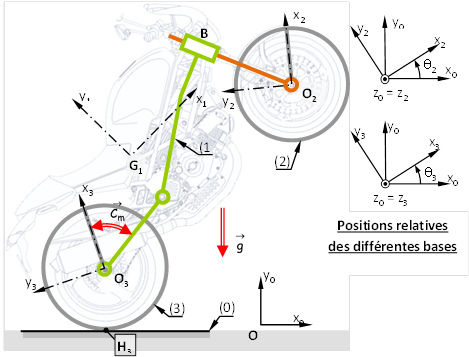
\includegraphics[width=\linewidth]{fig_01}
\end{marginfigure}

La figure ci-dessus représente un dispositif conçu pour déterminer le moment d'inertie $I$ d'un solide de révolution \textbf{(2)} par rapport à son axe. Soit $R_0$ un repère galiléen lié au bâti \textbf{($S_0$)} tel que l'axe $\axe{O}{x_0}$ soit vertical descendant. Les deux portées sur lesquelles roule le solide \textbf{(2)} sont des portions de la surface d'un cylindre de révolution d'axe $\axe{O}{z_0}$ et de rayon $r$.
Le solide \textbf{(2)}, de masse $m$, de centre d'inertie $C$, possède deux tourillons de même rayon $a$. Soit $f$ le coefficient de frottement entre \textbf{(2)} et \textbf{($S_0$)}.
L'étude se ramène à celle d'un problème plan paramétré de la façon suivante :
\begin{itemize}
\item le tourillon de \textbf{(2)}, de centre $C$, roule sans glisser en $A$ sur la portée cylindrique de \textbf{($S_0$)};
\item $R_1$ est un repère tel que $\vect{OA} = r\vect{x_1}$ et on pose $\theta=\angl{x_0}{x_1}$;
\item $R_2$ est un repère lié à 2 avec $\varphi=\angl{x_1}{x_2}$. On suppose que $\varphi = 0$ lorsque $\theta=0$.
\end{itemize}
\question{Donner la relation entre $\varphi$ et $\theta$.}
\question{Déterminer l'équation du mouvement de \textbf{(2)} par rapport à \textbf{($S_0$)} en fonction de $\theta$.}
\question{On suppose que l'angle $\theta$ reste petit au cours du mouvement. Montrer que le mouvement est périodique et déterminer la période $T$ des oscillations de \textbf{(2)}.}


\ifprof
\else
\begin{marginfigure}
\centering

\includegraphics[width=3cm]{Cy_04_02_Colle_PFD_02_MesureInertie_qr}
\end{marginfigure}
\fi

\question{En déduire le moment d'inertie $I$ de \textbf{(S)} sachant que :
$T=\SI{5}{s}$; $a =\SI{12,5}{mm}$; $r = \SI{141,1}{mm}$; $g = \SI{9,81}{m.s^{-2}}$;	$m = \SI{7217}{g}$; $f = 0,15$.}

\question{Déterminer l’angle $\theta_0$ maxi pour qu’il n’y ait pas glissement en $A$. Faire l’application numérique.}


\ifprof
%
\begin{center}
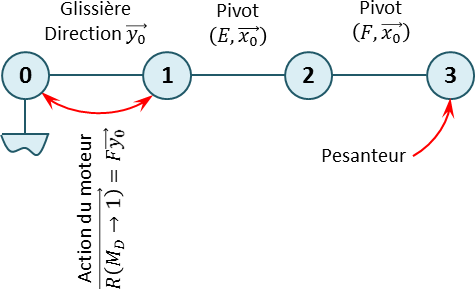
\includegraphics[width=\linewidth]{cor_01}
\end{center}
\begin{center}
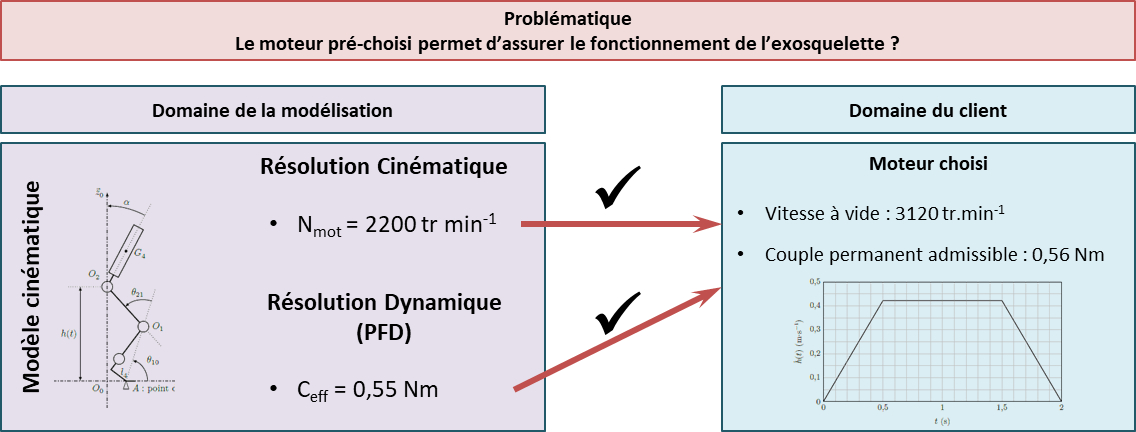
\includegraphics[width=\linewidth]{cor_02}
\end{center}

\else
\fi
